%%
%% Copyright 2007, 2008, 2009 Elsevier Ltd
%%
%% This file is part of the 'Elsarticle Bundle'.
%% ---------------------------------------------
%%
%% It may be distributed under the conditions of the LaTeX Project Public
%% License, either version 1.2 of this license or (at your option) any
%% later version.  The latest version of this license is in
%%    http://www.latex-project.org/lppl.txt
%% and version 1.2 or later is part of all distributions of LaTeX
%% version 1999/12/01 or later.
%%
%% The list of all files belonging to the 'Elsarticle Bundle' is
%% given in the file `manifest.txt'.
%%

%% Template article for Elsevier's document class `elsarticle'
%% with numbered style bibliographic references
%% SP 2008/03/01

\documentclass[preprint,12pt]{elsarticle}

%% Use the option review to obtain double line spacing
%% \documentclass[authoryear,preprint,review,12pt]{elsarticle}

%% Use the options 1p,twocolumn; 3p; 3p,twocolumn; 5p; or 5p,twocolumn
%% for a journal layout:
%% \documentclass[final,1p,times]{elsarticle}
%% \documentclass[final,1p,times,twocolumn]{elsarticle}
%% \documentclass[final,3p,times]{elsarticle}
%% \documentclass[final,3p,times,twocolumn]{elsarticle}
%% \documentclass[final,5p,times]{elsarticle}
%% \documentclass[final,5p,times,twocolumn]{elsarticle}

%% For including figures, graphicx.sty has been loaded in
%% elsarticle.cls. If you prefer to use the old commands
%% please give \usepackage{epsfig}

%% The amssymb package provides various useful mathematical symbols
\usepackage{amssymb}
\usepackage{caption}
\usepackage{slashbox}
\usepackage{graphics} % for pdf, bitmapped graphics files
\usepackage{epsfig} % for postscript graphics files
\usepackage{epstopdf}
\usepackage{subfig}
\usepackage{mathptmx} % assumes new font selection scheme installed
\usepackage{amsmath} % assumes amsmath package installed
\usepackage{array}
\usepackage{bm}

%\usepackage[noend]{algpseudocode}
%\usepackage{fancybox}
%\usepackage{alg}
%\usepackage{newalg}
%\usepackage{program}
%\usepackage[cmex10]{amsmath}
%\usepackage{times} % assumes new font selection scheme installed


\usepackage{hyperref}

%\usepackage[]{algorithm2e}
\usepackage{algorithm}
%\usepackage{algorithmic}
\usepackage{algpseudocode}
%\usepackage{fontspec}
%\usepackage[noend]{algpseudocode}

\journal{Journal of Robotics}

\begin{document}

\begin{frontmatter}

%% Title, authors and addresses

%% use the tnoteref command within \title for footnotes;
%% use the tnotetext command for theassociated footnote;
%% use the fnref command within \author or \address for footnotes;
%% use the fntext command for theassociated footnote;
%% use the corref command within \author for corresponding author footnotes;
%% use the cortext command for theassociated footnote;
%% use the ead command for the email address,
%% and the form \ead[url] for the home page:
%% \title{Title\tnoteref{label1}}
%% \tnotetext[label1]{}
%% \author{Name\corref{cor1}\fnref{label2}}
%% \ead{email address}
%% \ead[url]{home page}
%% \fntext[label2]{}
%% \cortext[cor1]{}
%% \address{Address\fnref{label3}}
%% \fntext[label3]{}

\title{Learning Human Manipulation Strategy by A Modular Approach}

%% use optional labels to link authors explicitly to addresses:
%% \author[label1,label2]{}
%% \address[label1]{}
%% \address[label2]{}

\author{}

\address{}
\begin{abstract}
Object manipulation is a challenging task for robot as the complicated physics involves in object interaction is hard to be expressed analytically. In this work we introduce a modular approach to learn the human manipulation strategy by demonstration. The human demonstrator demonstrated the task in different contexts and we group these demonstrates according to their control strategies. Forward and inverse model pairs are learnt from each group to encode the motor control policy. We validate our approach on a robot platform with a opening bottle cap task. We show that our approach can correctly identify the number of modules of a given task and generate proper motor commands for the robot to accomplish the task.
\end{abstract}

\begin{keyword}
Learning \sep Human demonstration \sep Multiple Modular \sep Manipulation
%% keywords here, in the form: keyword \sep keyword

%% PACS codes here, in the form: \PACS code \sep code

%% MSC codes here, in the form: \MSC code \sep code
%% or \MSC[2008] code \sep code (2000 is the default)

\end{keyword}

\end{frontmatter}

%% \linenumbers

%% main text

\section{Introduction}
\label{intro}
The ultimate goal of robotics is to enable robots to be a part of human life, to provide assistance in a wide range of tasks including surgery operation, house keeping, education and personal care. Most of these tasks require the ability to do complex object manipulation, which remains a open challenge in the robotics community. %It is impractical to pre-program all such object manipulation tasks manually. Therefore, we use a more practical alternative: teaching the robots by human demonstrations of the tasks.

Object manipulation is a large category of tasks in which the robots make physical contact with the environment. %Typical contact tasks include robot grasping and object manipulation.
The complicated physics in the interactions between objects makes it difficult.
In manipulation tasks, the ability to predict and react to the uncertainty and unforeseen changes of the environment is vital. The changes of the environment can be abrupt due to the multi-body interaction and the effect of friction. To handle these situations, robots have to be equipped with a nonlinear and non-stationary control strategy.

%TODO Human are experts in daily object manipulation tasks and reacting to a nonlinear and non-stationary changing environment. In this work, we adopt a program by demonstration(PbD)~\cite{schaal2003computational} approach to learn human control strategies of object manipulation.

%One of the classical adaptive control methods for a non-stationary system is fitting open parameters of a pre-defined parametric model. Fitting open parameters is not an easy task, it assumes the parameters change gradually. Hence this method is inadequate for control in manipulation tasks.



%In an object manipulation task the robot end effectors interact with the outside environment and hence causes changes of the environmental kinematic and dynamic configurations. Usually involving the effects of the friction between objects, these changes are abrupt (e.g. switching from static friction to kinematic friction) and highly nonlinear (e.g. interaction between multi-body). 
%Hence classic adaptive control methods, that assume gradual environment changes and allow large error during the period of adaptation, are inadequate for object manipulation.
%To handle these abrupt changes in the environment dynamics, a modular approach is more suitable as it allows rapid changes of strategies. %The multiple models approach is not new in adaptive control~\cite{narendra1997adaptive}. In a multiple models approach, we can evaluate the responsibility of each model according to the current status of the system dynamics to produce a mixing result.
%

%Human are experts in daily object manipulation tasks and reacting to a nonlinear and non-stationary changing environment.  In this work, we adopt a program by demonstration(PbD)~\cite{schaal2003computational} approach to learn human control strategies of object manipulation.

%Neuroscientists propose that animal have a modularized central nervous system~\cite{??}.
%Previous studies have provided evidence which shows that the human central nervous system uses a number of internal models of the system dynamics to control the motors of the body in different environments~\cite{wolpert1998multiple}. This hypothesis has been used to explain human predictive control and size illusion~\cite{??}. % We propose a methodology of doing so in this paper. %Robots learning human internal models from task demonstration is rarely discussed in literature.

The excellent manipulation skill of human is long desired by roboticists. Without using theoretical knowledge of the dynamics of the complex environment, human can manipulate objects easily. The fact that human have no difficulties in controlling their limbs under changes of the environment suggests that the brain use more than one models~\cite{haruno2001mosaic}. This inspires us to learn the internal models that human use for manipulation.

In this work, we introduce a modular approach to learn human internal models for manipulation. Modular approach has been shown to be an effective way of building intelligent systems~\cite{bryson2004modular,BrysonMcG12}. Our approach identifies a set of control strategies from human demonstration, each adapted to different task contexts. When a robot executes a task, it carries out an automatic estimation of the task context based on the sensory data and calculates a best combination of the modules to provide a motor command of the current operating region. The approach does not require any prior knowledge of the kinematics nor dynamics of the operation system, nor is it restricted to a specific robot platform. %The control strategy is learnt on the object level and hence can be transfer from human to robot directly.

We verify this approach experimentally by learning a specific task: opening bottle caps. This is a complex manipulation task as the friction between the contact surfaces has multiple phases of which the physics behind is not completely understood. Without detail knowledge of tribology, human is able to open many different bottle caps using adaptive control strategy. We learn this strategy by our modular approach. The robustness of the learnt control strategy is confirmed by applying it to open different bottles including unseen bottles. We show that our method simplifies the learning of a control strategy and can benefit a wide range of tasks.


The rest of the paper is organized as follows: Section~\ref{sec:related} provides an overview of the related work in literatures that motivate this work; Section~\ref{sec:method} introduces our approach of learning a multiple module model of human manipulation strategy; an experiment of a opening bottle cap task and its result is shown in Section~\ref{sec:exp}, along with details of the hardware specifications and the experimental setup; Section~\ref{sec:diss} concludes and discusses the contribution of this work, as well as proposes directions for future study.

\section{Related Work}
\label{sec:related}
In this section, we review related literature in the area of robot learning and human motor control.


\subsection{Robot learning}
\label{sec:imitation}
Demonstration based has been an active topic of research in the last decade. It speeds up robot learning with the demonstrator showing the constraints of the tasks.
%This approach has been studied in many different tasks~\cite{calinon2007learning,huang2013learning,hsiao2005imitation,Hueser06,kulic2012incremental,Ekvall07,wu2010hierarchical.}
Different from the classical manually programming approach, that relies on human insights of the dynamics of the tasks, this approach automatically generate models to encode the information extrated from demonstrations. Demonstrations provide the key features and constraints of the tasks, that can not be easily deduced analytically. This method has been extensively used in the tasks of body gesture reproduction~\cite{hsiao2005imitation,calinon2010learning,kulic2012incremental} and reaching motion planning~\cite{Ekvall07,shukla2012coupled,mohammad2014learning}, of which the large searching space is greatly reduced by using the demonstrations to suggest possible solutions. Besides this, demonstration based learning is also used in manipulation tasks~\cite{petkos2006learning,sauser2011iterative,Miao2014}, in order to transfer human knowledge in interacting with the environment to robot.

In order to capture information from demonstrations, different sensors are used for different tasks. Motion capture systems and data gloves are used to provide demonstrators' end effectors and joints' position information~\cite{calinon2007incremental,asfour2008imitation,kulic2012incremental,bidan2013robio}. Force torque sensors and tactile sensing systems are used to provide information about demonstrators' exerting force on the environment~\cite{sauser2011iterative,Miao2014}. 

The task information captured from sensors is needed to be transferred to robots. The different in the sensory and motor system of human and robot causes the correspondence problem.
%these task knowledge from human to robot, the correspondence problem caused by the embodiment difference between human and robots has to be solved. 
To solve this problem, different mapping methods are proposed in many literatures~\cite{asfour2008imitation,koenemann2012whole,kulic2012incremental}, while human correction~\cite{calinon2007incremental,sauser2011iterative,romano2011human} and self-correction~\cite{bidan2013robio} via learning are proposed as alternative solutions. Kinesthetic teaching~\cite{korkinof2013online,pais2014encoding} and tele-operation~\cite{Fischer98} are used to directly demonstrate a task on a robot and hence avoid the correspondence problem.

In object manipulation tasks, the object centric viewpoint~\cite{okamura2000overview} considers a manipulation task only from the object's perspective, which suggests the goal of learning a task is to reproduce the same object behaviour. Taking this principle, an object level approach is proposed in~\cite{Miao2014} to learn object impedance in grasping and manipulation tasks. Our approach takes the same principle and learns the human strategy to operate the objects that will produce the same object behaviour.

All the these approaches obtain task information from human demonstrations. To make the best use of human knowledge, the information should be encoded in a similar way that human encode it. Human tactile sensation scheme is implemented to robot for grasping control and result in a good performance~\cite{romano2011human}. However this approach of using human motor control mechanism to build models of tasks is rarely discussed in literature.


%Physical interaction between the robot and the environment is one important characteristics of manipulation tasks, the problems rise from the complicated physics in the interactions between objects is hard to solve analytically. Without using detail knowledge of multi-body dynamics nor tribology, however, human can manipulate objects without difficulties. To learn human manipulation strategies

% While learning body gestures and reaching target strategies mainly use motion tracking systems to read the demonstrators'
%While learning in position control~\cite{calinon2010learning,kulic2012incremental} has been extensively studied, learning in force/impedence control is less discussed in literatures~\cite{sauser2011iterative,petkos2006learning}. In manipulation tasks, force control is an important method as force produce direct impact to the environment.

%\subsection{Manipulation task}
%\label{sec:manipulationtask}

\subsection{Human motor control}

In the study of human motor control, internal model is one of the most evidently supported hypothesis. It postulates a neuron process that simulates output of the motor system and the environment~\cite{kawato1999internal}. It's applications in robot control have been explored by many researchers. Various types of internal models are built for different tasks~\cite{sciavicco2000modelling,jordan1992forward}.

The excellent ability of human to manipulate different objects in different contexts and quickly adapt to change of contexts suggested that our central nervous system (CNS) maintains multiple internal models of outside environments, rather than a single internal model that adapts to new environment~\cite{neilson1985acquisition}. Based on the concept of modularity, the Modular selection and identification for control (MOSAIC) architecture was proposed to explain the motor control strategy of the CNS~\cite{wolpert1998multiple}. According to this hypothesis, during the motor control process, the brain quickly select the most appropriate modules according to the current environment context and use them to generate an appropriate motor command to react to the environment~\cite{haruno2001mosaic}.

The benefit of this multiple model approach has been long discussed in the control community~\cite{jacobs1991adaptive,narendra1995adaptation,narendra1997adaptive}. Some recent works~\cite{fekri2007robust,kuipers2010multiple} present promising modular based approaches. Multiple model approach also has a wide range application in robot control. It is particular useful for tasks in nonlinear and non-stationary environment~\cite{petkos2006learning,sugimoto2012emosaic}



The approach we take is a modular approach inspired from MOSAIC~\cite{haruno2001mosaic}. In our approach, the human control strategy is encoded by multiple pairs of forward and inverse models. The final motor command is the linear combination of the commands generated from each inverse models factored by their weights estimated by the forward models. The linear combination, rather than switch, of the models requires less number of modules to approximate the system dynamics. Indeed, neuroscience evidence suggests that animal brain sum modular stimulates of muscles to generate different motions~\cite{mussa1994linear}. To the best of our knowledge, this is the first realization of the multiple module model in an object manipulation task with a real robot, learnt from human demonstration.

%It is particularly useful to use learning to approximate internal models for motor control when the analytical model of the system dynamics is not easy to deduce.
%
%
%%Though the MOSAIC has gained a large concerns in neuroscience community, this approach is not widely used in robot control.
%
%Imitation learning has been an active topic of research in the last decade. It speeds up robot learning with the demonstrator showing the constraints of the tasks.

%The approach we take is a modular approach inspired from MOSAIC~\cite{haruno2001mosaic}. In MOSAIC, each dynamic system context is encoded by a pair of forward and inverse models. At each time step, the forward models estimate the current context and compare it with the actually context. The accuracy of the estimation decided the weight of the corresponding inverse models. The final motor command is the linear combination of the commands generated from each inverse models factored by their weights. The linear combination, rather than switch, of the models requires less number of models to approximate the system dynamics. Indeed, neuroscience evidence suggests that human brain mix modular stimulates of muscles to generate new motions. Our work focus on learning human's strategy of adaptive control on a modular base. To the best of our knowledge, this is the first realization of the multiple model control in an object manipulation task with a real robot, learnt from human demonstration.
%It can be used for solving nonlinear and non-stationary control problem.



%learning from human demonstration approach.


%
%Scientist has long been fascinated by human adaptive motor control ability and wondering the mechanism of it. One of the most evidently supported hypothesis is the multiple model~\cite{neilson1985acquisition}. %~\cite{haruno2001mosaic}


(TODO: Joanna thinks this part can be extended. Please feel free to add any literatures that you think should be included. )


\section{Methodology}
\label{sec:method}
% ========= object centric =========
Our goal is to acquire a modular based control policy for an object manipulation task from human demonstration. To this end, we take a three-step approach:
\begin{enumerate}
\item Human demonstrating a task in different contexts (Section~\ref{sec:demo}).
%\item Clustering the data to find number of modules needed in the task (subsection ~\ref{sec:cluster}).
\item Learning a multiple module model to encode human control strategies (Section~\ref{sec:learn}).
%\item Design a controller based on the learnt multiple model  (subsection ~\ref{controller}).
\item Use the multiple module model to compute motor commands (Section~\ref{sec:command}).
\end{enumerate}


\subsection{Human demonstration}
\label{sec:demo}

\begin{figure}
  \centering
  \includegraphics[width=5cm]{./fig/ravin.jpg}
  \caption{ \scriptsize{Human demonstration of opening a bottle cap.}
}
\label{fig:demo}
\end{figure}

The first step is recording human demonstration of a task. Based on the object centric principle, we collect the object trajectory and its driven force. These data can be accessed by motion capture system, force-torque sensor and wearable haptic device(Fig.~\ref{fig:demo}).

% ===== Why not kinematics approach? =====
For manipulation task, kinematics teaching on robot is difficult. While a manipulation task usually involves multifinger movement, a human can kinematically operate one finger with each hand and hence two fingers simultaneously for the most extend. Tele-operation of the robot hand solves this problem but it does not provide a direct force feedback. In our approach, human perform the task with direct interaction with the object. With direct interaction with the object the teacher is able to perform the task most naturally and perform a more delicate control strategy. %In an object centric manner there is no difference between collecting data from the teacher or from the learner -- they are expressed from the objects' perspective. Once the control policy is encoded, it can be directly applied to the robots.

%Kinematics teaching of the learner is not necessary here for three reasons. Firstly in an object centric manner there is no difference between collecting data from the teacher or from the learner -- they are expressed from the object point of view. Secondly with direct interaction with the object the teacher is able to perform the task most naturally and hence provide a more naturally control policy. Thirdly manipulation with multifinger is difficult to demonstration kinematically, as a human can manipulate one finger of a robot with each hand and hence two fingers simultaneously for its most extend.

% ======= demonstrate in different context =======
In the demonstration, the teacher perform a task a number of times to generate enough data for capturing the key features of it. Further, the teacher perform the task under different system kinematics and dynamics configurations, e.g. friction conditions, in order to explore how human adaptive to different task contexts. These different configurations are chosen to cover a wide range of different contexts. For example, in a opening bottle cap task the demonstration of opening the tightest bottle, within the capability of the learner, is included. Details will be explained in Section~\ref{sec:exp_demo}.
%How to cover ??????


%The force and torque applied on the cap are measured by the Trkscan pressure sensor and a force torque sensor. The movement of the object is recorded by the OptTrack motion tracking system. Each demonstration is recorded as a temporal sequence.

%~\cite{bidan2013robio}
%~\cite{huang2013learning}
%~\cite{huanghumanoid}
\subsection{Learning a Multiple-Module Model}
\label{sec:learn}
In this section we detail our modeling method, explaining how do we model human manipulation strategy and how to choose the number of modules of a task.

\subsubsection{Object centric manipulation strategy}
\label{sec:objectlevel}
As mentioned in Section~\ref{sec:related}, one of the challenges in imitation learning is the correspondence problem, i.e. how to map the teacher's motions to the robot's motions so that they produce the same effects, e.g. reaching the same point. %This problem is particularly important in the motion planning tasks.
In a object manipulation task, however, the goal is to deliver the object from the current state to a desired state. During this process the movement of the manipulator is bounded by the movement of the object. It is more important to imitate how human apply forces to achieve object's desired movement, than to imitate the human limb movement. 
%Therefore we take an ``object centric approach"~\cite{okamura2000overview}, of which the control policy is taken from the object point of view. 

Therefore, our model encodes a force and torque profile rather than the end effector movement trajectory. The imitation learning objective here is not to find a policy for the end effector movement but to find a policy that maps the force and torque to the object movement. This policy allows the robot to efficiently acquire new behaviors to accomplish the task. %Different robots move differently to achieve the desired object movements. 
Giving the robots' kinematics and the desired exert force on the object, the joint torques can be deduced by the Jacobian matrix~\cite{okamura2000overview}. To this end, we focus on the force-torque-displacement tuple: $\{F,\tau,s\}$ demonstrated in the task. In later sections, we refer $\{F,\tau\}$ as the motor command with notation $\{a\}$. In each demonstration, a time series of the tuple is recorded.



\subsubsection{Decide number of modules}
\label{sec:cluster}

% ----------- why clustering -----------
Due to the involvement of object interaction, a manipulation task frequently encounter abrupt changes of the system dynamics, e.g. transfer between status of no contact to contact, of static friction and dynamic friction. Different strategies should be used to handle different dynamics. We achieve this goal by using a modular approach. Multiple modules are learned from the demonstrations under different task contexts. %During implementation, the system quickly estimate the context by the sensory inputs and choose the most appropriate module or weight and combine the modules to react.

%In this multiple model approach, each model is trained for a particular dynamics context. During the control process the model can compute appropriate control commands for the corresponding dynamics according to the sensory inputs. If the model is chosen properly (see Section~\ref{rf} for mixing model), this approach will be able to adapt to changing environmental context.

% ---------- Cluster to find number of modules -----------
Different tasks may need different number of modules. In human demonstration the same task is demonstrated with a few different setups to explore how human adapt to them. However, the number of setups does not necessary equal to the number of modules needed in the task. Human may handle a few different contexts with the same control strategies. %Some data may seems to be dissimilar in the scale or frequency, but in fact are governed by the same dynamic.
In order to find a proper number of modules, we need to differentiate different types of strategies. The differences can be reflected from the different pattern of the force-torque-displacement tuple. Hence we differentiate the patterns in a data driven manner: cluster force-torque-displacement tuple. Data in the same cluster is considered to be governed by the same strategy. The number of clusters is the number of modules and each module is encoded by one model.


% ----------- Distance Metric for clustering ------------
The goal of clustering is to separate a set of data to a few groups according to their similarities. The first step of clustering is to measure the similarities, i.e. the distances, between different data points. Different from an usual clustering problem, the data we need to cluster are not a set of single data points but a set of time series. Here we use the Dynamic Time Warping technique (DTW) to measure the distance between each pair of time series.

Dynamic time warping is suitable for measuring the similarity between two time series, which may have different speeds or durations. It warps the data in the time dimension and finds the optimal match between the time series. The similarity is computed as the average distance between the corresponding points in two series.

The similarity (distance) between each pair of time series is computed by DTW and produce a distance matrix. In this distance matrix, each element contains a measurement of the similarity between two time series. We then cluster these time series into a few groups by a threshold of the similarity. This threshold is set by using the variance of the data from the same context as a reference. As mentioned above, under the same context a task is demonstrated a few times. These demonstrations are presumed to be handled with the same strategy and hence belong to the same cluster. The variance of these demonstrations give a reference of a proper variance of a cluster. The largest variance, across the variance of all contexts, is used as the threshold for the clustering.

%% ------------ Hierarchical clustering -----------
Without knowing the number of clusters at the first place, we use an hierarchical agglomerative clustering method. Agglomerative clustering is a method that merges data iteratively until the stop criteria satisfied, which does not require a predefined number of clusters. Our clustering method is described as follow:

\begin{enumerate}
\item At the beginning, each single time series is considered to be one cluster.
\item Compute the distances between each pair of clusters.
\item Starting from the first cluster, find its nearest cluster. We define the distance between two clusters to be the average distance across all the time series pairs in them. If the distance to the nearest cluster is smaller than the threshold, merge these two cluster.
\item Move to the next cluster. Repeat the last step for the rest of the clusters.
\item A new set of clusters are formed by the last few steps, move to the next hierarchy and repeat the step 2 to 4 until no new clusters can be formed.
\end{enumerate}

Pseudocode of the complete algorithm is shown in Algorithm~\ref{code:cluster}.

\begin{algorithm}
  \caption{Agglomerative Hierarchical Clustering}
  \begin{algorithmic}[1]
%    \Require{$x$ and $y$ are packed strings of equal length $n$}
%    \Statex Init();
    \State Init(): Make each time series a cluster\;
    \State $mergeable$ = true\;
    \Function{Merge}{all clusters, distance matrix} %      \Comment{$\oplus$: bit}
    \While{mergeable is true}
      \State $mergeable$ = false\;
      \For{each cluster}
        \State $ClusterA$ = current cluster\;
        \State $ClusterB$ = nearest neighbor of $ClusterA$\;
        \If{distance($ClusterA, ClusterB$) $<$ clustering threshold}
            \State Merge $ClusterB$ into $ClusterA$\;
            \State $mergeable$ = true\;
        \EndIf
      \EndFor
      %\State \Return{$\delta$}
    \EndWhile
    \EndFunction
  \end{algorithmic}
  \label{code:cluster}
\end{algorithm}



% --------- Number of cluster -----------
When the clusters can not be merged further, we discover the number of modules require in this task: it is the number of the remaining clusters. Each cluster is used as a module. The pattern of the data in a cluster represents a strategy of handling specific task contexts.

\subsection{Learning Models}
\label{sec:model}
After identifying the number of modules, we build models for each of the module. In this section, we explain the way we encode human manipulation strategy.

During demonstrations, we constantly acquire the object displacements and the force and torque applied by the teacher. The teacher is the only source of exert force and torque of the system. The relationship between the exert force and torque and their resulting object displacement shows the dynamic characteristic of the task. A classic way to describe the system behaviour is using impedance. Giving a desired impedance of a task, we can compute a proper motor command for the robot to accomplish the task. %These two types of models have common drawbacks in modeling a manipulation task.
However the impedance is usually hard to specified in a given task, especially for task involving varying impedance. Most of the time it is roughly approximated by a linear model. As a result, impedance control are usually effective in slow changing and linear tasks. Specification of the impedance of a nonlinear task remains a open problem.

%GMM
In our approach, we model the correlation of the force and the displacement rather than estimating the impedance. To this end, we use the Gaussian Mixture Model (GMM)~\cite{cohn1996active}. The task dynamics is encoded as a joint distribution of the object status displacement $s$ and the action $a$ taken by human $p(s,a,{\mid}{\Omega})$.
Modeling the distribution by GMM allows us to capture the nonlinearity in the data. Further more, as a generative model it also allows us to compute the likelihood of a query data point in the model. This provides an good estimation of the reliability of the module in the current task context, which is crucial in choosing the correct modules for control (discussed in Section~\ref{sec:rf}).

With a GMM, the joint distribution of the variables is expressed as a sum of N Gaussian components,
\begin{equation}
{
p(s,a\mid\Omega)
= \sum_{n=1}^N {p_{n}p(s,a\mid{\mu}_n},{\Sigma}_n)
}
\end{equation}
where $p_n$ is the prior of the $n$-th Gaussian component and the ${\mu}_n$, ${\Sigma}_n$ the corresponding mean and covariance as:

\begin{equation}
{
{\mu}_n = \begin{pmatrix}    {\mu}_{s,n}     \\
                             {\mu}_{a,n}          \\
                    \end{pmatrix}
\hspace{0.2in}
{\Sigma}_n = \begin{pmatrix}     {\Sigma}_{ss,n}  &
                                 {\Sigma}_{sa,n} \\
                                 {\Sigma}_{as,n}  &
                                 {\Sigma}_{aa,n}   \\

                        \end{pmatrix}
}
\end{equation}

%The choice of GMM give us three advantages. Firstly, it is good in modeling nonlinear behavior. Secondly, it tolerates noisy of the data in a good extend and give good estimation of the expected values. Thirdly, as a generative model, it allows the computation of the likelihood of a given input data in the model. This provides an easy measurement of the reliability of the module, which is crucial in choosing the correct modules for control (see Section~\ref{sec:rf}).

%We use the Gaussian Mixture Model (GMM)~\cite{cohn1996active} to encode the task dynamics, and get a joint distribution of the object status $s=\{(x^t,v^t)\}^T_{t=1}$ (displacement $x$ and velocity $v$) and the action taken by human ($a=\{f^t,\tau^t\}^T_{t=1}$) $p(s, a, {\mid} {\Omega})$. The choice of GMM give us three advantages. Firstly, it is good in modeling nonlinear behaviour. Secondly, it tolerates noisy of the data in a good extend and give good estimation of the expected values. Thirdly, as a generative model it is flexible of the type of control: we can compute the force and torque from the given displacement and velocity or compute the displacement and velocity from the given force and torque. %According to different tasks, the variables encoded by GMM may be in different format, e.g. for multi-step prediction control we need to model $s$ in the form of $s=\{x^t,x^{t-1},x^{t-2},...,v^t,v^{t-1},v^{t-2},...\}$. See later section~ref{experiment} for details.


We aim to build a model closely simulates human motor strategy in order to make the best use of the human data. Evidences of neuroscience suggest that human develop internal model for motor control, so as to estimate the outcome of a motor command. The use of internal model speed up the human correction and reaction in motor control. One hypothesis of the internal model is MOSAIC, which is a multiple modular model composed by a couple of pairs of forward model and inverse model. We build our control strategy based on this hypothesis.

A forward model is held to anticipate the outcome of the motor command, while an inverse model is held to generate motor commands to take the current system state to the next state. The discrepancy between the anticipation of the forward model and the actual feedback is used to correct the motor command generated from the inverse model (Section~\ref{sec:rf}). Figure~\ref{fig:control} shows the basic control flow of a forward-inverse model pair.

\begin{figure}
  \centering
  \includegraphics[width=10cm]{./fig/control_1.jpg}
  \caption{ \scriptsize{Control flow diagram of forward-inverse model in motor control.}
}
\label{fig:control}
\end{figure}

% ----------- One model for both -------------
%The internal model ${\Omega})$ (forward model and inverse model) is encoded by the joint distributions of the variables, i.e. $p(s_t,s_{t+1},a_{t-1},a_t\mid{\Omega})$. This joint distribution encodes the forward model and the inverse model at the same time and both of their functionalities can be realized by the Gaussian Mixture Regression (GMR). For a given previous state and previous motor command, GMR provides a close-form solution to compute the anticipating state $s_t$, i.e. $p(s_{t+1}{\mid}s_{t},a_{t},{\Omega})$. For a given current state and desired state, we can compute the motor command using GMR, i.e. $p(a_t{\mid}s_t,s^{*}_{t+1},{\Omega_f})$. In some tasks, the initial status of the system remains unchanged for a certain time until the exert force or torque is big enough to change it. This will cause degeneracy in the inverse model. To solve this problem we include the previous motor command into the model, i.e. $p(a_t{\mid}s_t,s^{*}_{t+1},a_{t-1},{\Omega_f})$.

% --------- one model for each ----------
The forward model $\Omega_I$ is encoded by the joint distributions of the current system state, previous system state and the previous motor command, i.e. $p(s_t,s_{t-1},a_{t-1}\mid{\Omega_I})$. For a given object displacement and a motor command, the Gaussian Mixture Regression (GMR) provides a close-form solution to compute the anticipating object displacement $s_t$, i.e. $p(s_t{\mid}s_{t-1},a_{t-1},{\Omega_I})$. The inverse model $\Omega_f$ is encoded by the joint distributions of the current object displacement $s_t$ and the desired object displacement $s^{*}_{t+1}$. In some tasks, the initial status of the system remains unchanged for a certain time until the exert force or torque is big enough to change it. This will cause degeneracy in the inverse model. To solve this problem we include the previous motor command into the model, i.e. $p(s_t,s^{*}_{t+1},a_{t-1},a_t{\mid}{\Omega_F})$.



% Non-linear, multi model. What to solve in multi model
%As discussed above, one of the characteristics of manipulation task is the changing kinematics and dynamics configuration.
%In different task contexts, the pattern of the correlation between the displacement and action may be different. 
By clustering the training data into different groups as discussed in Section~\ref{sec:cluster}, we are able to discover the number of different patterns, i.e. number of modules. We train one GMM on each of the modules to encode the different changing patterns of the task context.


% Learn system dynamics, impedance, admittance.

%Phases
%A single model is usually not enough to encode all these different configurations. Therefore we adopt a multiple modular approach to model the different environment. There are two key problems needed to be resolve in a multiple modular approach: how many models to build (Section~\ref{cluster}) and how to weight the models during the control process (Section~\ref{rf}).




\subsection{Multiple modular adaptive control}
\label{sec:control}
%% forward-inverse modeling
%%After clustering the data into different groups, we train each cluster with the GMM $p(X_T, X_{t+1}, U_{t-1}, U_t {\mid} {\Omega})$.
%We model each of the cluster to encode the human control policy under different dynamics.
%Neuroscientists suggested that human use a mixture of forward model and inverse model for motor control. The forward model
%With the learned multiple models, we adopt the MOSAIC~\cite{haruno2001mosaic} architecture to control the system. The basic concept of MOSAIC is that the human brain use multiple inverse models to control the system, which is augmented with a forward models. In human brain there exist multiple pairs of coupled forward and inverse models. The forward models estimate the reliability of the inverse model in the current context, and the final motor command is a linear combination of all the commands from the inverse models.
%In object manipulation, the system dynamics can be rapidly changing over time and we need more than one model to describe it. Our learnt multiple GMMs are used to describe the system in these different contents. First we need to infer the behavior of the system. Having deduced this information, we need to decide how to manipulate the system.

Once the number of modules is found and the multiple pair of forward and inverse models are learnt, they are used to compute motor commands for task execution.
We consider the human motor system acts upon by motor command $a_t$ at time $t$ with current system status $s_t$. The resulting system status at time $t+1$ then is

\begin{equation}
\label{e1}
s_{t+1} = f\left(s_t,a_t\right)
\end{equation}

The goal of the controller is to generate a motor command that bring the current system status from $s_t$ a desired state $s^*_{t+1}$:

\begin{equation}
\label{e2}
a_t = g\left({s^*_{t+1},s_t}\right)
\end{equation}

According to the discussion in Section~\ref{sec:model}, equation~\ref{e1} represents the forward model and equation~\ref{e2} represents the inverse model. It takes three steps to compute the motor command $a_t$:
\begin{enumerate}
\item Compute expected system state $\hat{s}_t$ by each forward model
\item compute responsibility factor $\lambda$ for each module
\item Compute motor command by each inverse model and compute the final motor command $a_t$
\end{enumerate}


\subsubsection{Anticipate sensory output by forward model}
\label{sec:forward}
With the $k$-th forward model we can estimate the current status $\hat{s}_t$ by
\begin{equation}
\label{e3}
\hat{s}^k_{t} = E\left({s_{t-1}, a_{t-1} \mid \Omega^k_I}\right)
\end{equation}

%and
%
%\begin{equation}
%\label{e4}
%u^i_t = E\left({x^*_{t+1},x_t, u^i_{t-1} \mid \Omega^i}\right)
%\end{equation}

%These two equations will be described later in details.
This equation is to predict the environment status based on the observation and prediction on the controller's influence on the system. The expectation values of the current system status of the $k$-th module is computed by the $Gaussian$ $Mixture$ $Regression$ (GMR). The computation is as follow.

With the sensory input $\{s_{t-1},a_{t-1}\}$ as a query point $q$ we define:

\begin{equation}
{
 {\mu}_{q,n}^k = \begin{pmatrix} {\mu}_{s_{t-1},n}^k    \\
                                        {\mu}_{a_{t-1},n}^k
                        \end{pmatrix}
\hspace{0.3in}
{\Sigma}_{qq,n}^k =  \begin{pmatrix} {\Sigma}_{s_{t-1}s_{t-1},n}^k  & {\Sigma}_{s_{t-1}{a_{t-1},n}}^k  \\
                                            {\Sigma}_{{a_{t-1}}{s_{t-1}},n}^k  & {\Sigma}_{{a_{t-1}}{a_{t-1}},n}^k
                            \end{pmatrix}
}
\end{equation}
and GMR then uses:

\begin{equation}
{
\hat{\mu}_{s_t,n}^k = {\mu}_{s_t,n}^k + \Sigma_{{s_t}q,n}^k({\Sigma}_{qq,n}^k)^{-1}(q-{\mu}_{q,n}^k)
}
\end{equation}

\begin{equation}
{
\hat{\Sigma}_{{s_t}{s_t},n}^k = {\Sigma}_{{s_t}{s_t},n}^k - {\Sigma}_{{s_t}q,n}^k({\Sigma}_{qq,n}^k)^{-1}{\Sigma}_{q{s_t},n}^k
}
\end{equation}


Finally, all the $N$ Gaussian components of the $k$-th module\footnote{Different modules may have different number of Gaussian components.} are taken into account and the current sensory data $\hat{s}_t$ is predicted as the mean $\hat{\mu}_{s_t}$ with the covariance $\hat{\Sigma}_{s_t,s_t}$ according to:

\begin{equation}
{
\hat{\mu}_{s_t} = \sum_{n=1}^N{\beta_n(q)}\hat{\mu}_{s_t,n}^k
}
\end{equation}
\begin{equation}
{
\hat{\Sigma}_{{s_t}{s_t},n} = \sum_{n=1}^N{\beta_n(q)}^2\hat{\Sigma}_{{s_t}{s_t},n}^k
}
\end{equation}
where
\begin{equation}
{
\beta_n(q) = \frac{p_{n}p(q|{\mu}_{q,n}^k,{\Sigma}_{qq,n}^k)}
{\sum_{n=1}^N{p_n}p(q|{\mu}_{q,n}^k,{\Sigma}_{qq,n}^k)}
}
\end{equation}



\subsubsection{Responsibility factor}
\label{sec:rf}

In a multi-module approach, choosing the proper modules to compute the motor command is crucial. For this we rely on the computation of the responsibility factor. The responsibility factors act as the weight of the modules. Each module has its responsibility factor at every time step, the final motor command at that time step is the linear combination of the commands generated from each module multiplied by their responsibility factors.
The responsibility factor is a measurement of the reliability of using one model to represent the current system contexts.
%The measurement is computed by the discrepancy between the anticipating current system state $s_t$ of the forward model and the actual current system state $s'_t$ from the sensory feedback:
%
%\begin{equation}
%\lambda'^j_t = {$s'_t$ - p(s_t{\mid}s_{t-1},a_{t-1},\Omega^j)}}
%\end{equation}
%
%where $n$ is the number of models.

As the models are built as GMMs, it is easy to estimate the likelihood of one data point belongs to a particular module. The actual current state from the sensory feedback, the previous state and the previous motor command forms a query point $\{s_t,s_{t-1},a_{t-1}\}$. The responsibility is computed by the likelihood of the current query data point in each module, normalized by the total sum:

\begin{equation}
\lambda^j_t = \frac{p(s_t,s_{t-1},a_{t-1}\mid \Omega_I^j)}{\sum_{k=1}^{K}{p(s_t,s_{t-1},a_{t-1}\mid \Omega_I^k)}}
\end{equation}
where $K$ is the number of modules.

%Note the forward model is embedded in this computation of the responsibility factor. The likelihood of the query point $p(s_t,s_{t-1},a_{t-1}\mid \Omega^j$ in the $j-th$ module is equivalent to the discrepancy between the expected current system state $s_t$ of the forward model and the actual current system state $s'_t$ from the sensory feedback, factorized by the variance of the forward model.

\subsubsection{Generate motor command by Inverse Model}
\label{sec:inverse}
%While the forward models predict the current status of the system by the previous status and motor commands, the inverse models generate the next motor command according to the current status and the next target status. In reality, given a current state and a desired state, the command bring the robot to the desired state is not unique. In addition, during object manipulation, it is often the case that the force applying on the object various but the object position does not change because of friction. Therefore we include the previous command into the query point in order to generate the next command without redundance. Hence the command generated by each model is computed by equation~\ref{e4}.
%\subsubsection{Mix of Model}
%\label{mix}

The motor command $a^k_t$ for the $i$-th inverse model is computed by GMR with the same steps  described in Section~\ref{sec:forward}. The responsibility factors $\lambda^j$ act as the weights of each model in the control system. The higher the responsibility is, the more response the model takes in the control system. Therefore, the final motor command generated by this multiple model system is

\begin{equation}
\label{e_mix}
s_t = \sum_{k=1}^K{\lambda^k a_t^k} = \sum_{k=1}^K{\lambda^k E\left({s^*_{t+1},s_t, a^k_{t-1} \mid \Omega^k_I}\right)}
\end{equation}

These three steps are computed with a close form solution. This ensures that this system can react quickly to the changes in the environment by adjusting the responsibility factor.





\section{Robot Experiment}
\label{sec:exp}
% Why others only in simulation? what can't be simulated? [sethu2005]
The proposed multiple model approach is implemented on a real robot system (the KUKA robot arm and the Barrett Hand) for a particular manipulation task: opening bottle caps. The target of this task is to unscrew a tighten cap. 
This task is chosen as it is a common task in human daily life and at the same time a complex one from the control point of view. 
Before the task begins, human does not possess any information about the tightness of the cap. During the task, human constantly update the motor commands, i.e. how much torque to apply to the cap and how much force to grip the cap, according to the sensory feedback of the status of the context. This plan can not be make in advance as the dynamic configuration of each bottle is different and it changes throughout the duration of the task. Human have to cope with these uncertainties and adapt to the changes. In the later sections, we will explain the experiment details and show that the multiple module approach is able to acquire human adaptive control policy and enable the robot to master this manipulation task.
%For an object manipulation task, it is hard to simulate as it involve friction between objects. Therefore we implemented this system on a real robot, the KUKA robot arm mounted with the Barrett hand. The task we are looking at is opening bottle caps.

\subsection{Human demonstration and experimental setup}
\label{sec:exp_demo}
%Fig.~\ref{setup} shows the setup of the human demonstration. %In this task we record 2 variables: the displacement of the cap and the torque driving the cap to run. We used the Optitrack motion tracking system to morning the position and orientation of the cap, a force torque sensor mounted on the bottle to measure the driving torque.

%\begin{itemize}
%\item Dry friction can induce several types of instabilities in mechanical systems which display a stable behavior in the absence of friction.
%\item For instance, friction-related dynamical instabilities are thought to be responsible for brake squeal and the 'song' of a glass harp,[33][34] phenomena which involve stick and slip, modeled as a drop of friction coefficient with velocity.[35]
%\item Lubricated friction/dry friction
%\item not always follow Coulomb's law
%\item extremely complicated physical interaction
%\item adhesive tape
%\end{itemize}

Opening bottle cap is a common task for human however a difficult one for robot. The friction coefficient between the bottle and the cap, and the way they change from screwed to unscrewed, vary among different bottles. This requires different controlling strategies to open different bottles. Hence a multiple module approach is suitable for this task, which includes at lease two different control strategies for the system governed under static friction and kinetic friction.

The task involves the control of the turning torque, griping force according to the displacement of the cap. As the changes of the friction coefficient is nonlinear during the unscrewing process, it is hard to build an analytical model for it. Human can easily open most of the bottles in daily life. Learning from human demonstration will allow us to gain a controlling strategy without writing the analytical expression of the dynamics of the whole system.

In each demonstration, data from first time the finger touch the cap to the cap is finally open and lifted was recorded. Opening bottle cap is a cyclic task. Each cycle includes three stages: reaching, turning and releasing. In our experiments, four to six cycles need to be completed to open the bottles. During the reaching and releasing stages, no torque nor griping force is applied to the cap and the cap remains still. During the turning stages, human continuously apply torque to the cap and it starts moving once the friction is overcome.

\subsubsection{Demonstration in different task contexts}
\label{sec:exp_context}
The experiment starts with human demonstration. In order to explore different task context, we demonstrated the task with different setups, which are the combination of four different bottles ($b1-4$) and four different caps ($c1-4$) (Fig.~\ref{fig:b_c}). According to the surfaces situation of the bottles and the caps, the difficulty of opening the bottles varies. We lubricate the cap and bottle surfaces of $b1$ to make it easy, and leave adhesive materials on the surfaces of $b4$ to make it difficult. $b1-4$ are labeled by increasing difficulty, while $c1-4$ are labeled by the increasing diameters of the caps.

%By the increasing order of the friction, the bottles are labeled as $b1$, $b2$, $b3$, $b4$ (in order to enlarge the variance of the friction coefficients, we put lubricant to the bottle $b1$ and rough the contact surface between the bottle and the cap of $b4$). By the increasing order of the diameters of the caps, they are labeled as $c1$, $c2$, $c3$ and $c4$.

We chose to vary the setups in friction coefficient and cap size as these are the main variances between different bottles effecting the control strategy. The intention is to see how does these two variables effect human behaviour. To this end, we ``combine'' the bottles and the caps by mounting the caps onto the ``actual caps'' of the bottles (Fig.~\ref{fig:setup}). In this way, we have seven different setups for the demonstration (Table~\ref{bottlesandcaps}). Demonstrations on the set of setups with the same cap and different bottles, i.e. $b1c2, b2c2, b3c2, b4c2$, allow us to explore human strategies in adapting to different friction coefficients. Demonstrations on the set of setups with the same bottle and different caps, i.e. $b3c1, b3c2, b3c3, b4c3$, allow us to explore human strategies in this task with different cap sizes which result in different grasping strategies.

\begin{figure}
  \centering
  \includegraphics[width=5cm]{./fig/b_c.jpg}
  \caption{ \scriptsize{Bottles and caps for human demonstration. From left to right: b1 c1, b2 c2, b3 c3, b4  c4}
}
\label{fig:b_c}
\end{figure}



%\begin{figure}
%\centering
%    \subfloat[\scriptsize{}]  {\includegraphics[width=0.8in]{./fig/spr.jpg}}
%    \hspace{0.07in}
%    \subfloat[\scriptsize{}] {\includegraphics[width=0.8in]{./fig/box123.jpg}}
%%    \hspace{0.01in}
%\caption{\scriptsize{(a) A spray flask. (b) A spray flask approximated by 3 boxes.}}
%\label{fig:spr}
%\end{figure}



\begin{table}
\center
\begin{tabular}{l |l l l l}

\backslashbox{Bottle}{Cap}      & \parbox[c]{1em}{ \includegraphics[width=1cm]{./fig/c1.jpg}}
                                & \parbox[c]{1em}{ \includegraphics[width=1cm]{./fig/c2.jpg}}
                                & \parbox[c]{1em}{ \includegraphics[width=1cm]{./fig/c3.jpg}}
                                & \parbox[c]{1em}{ \includegraphics[width=1cm]{./fig/c4.jpg}}  \\
    & Cap 1& Cap 2& Cap 3& Cap 4\\
\hline
\parbox[c]{1em}{ \includegraphics[width=1cm]{./fig/b1.jpg}} & & &b1c3 &\\
Bottle 1 & & & &\\
\hline
\parbox[c]{1em}{ \includegraphics[width=1cm]{./fig/b2.jpg}} & & & &\\
Bottle 2 & b2c1& b2c2& b2c3& b2c4\\
\hline
\parbox[c]{1em}{ \includegraphics[width=1cm]{./fig/b3.jpg}} & & & &\\
Bottle 3 & & & b3c3&\\
\hline
\parbox[c]{1em}{ \includegraphics[width=1cm]{./fig/b4.jpg}} & & & &\\
Bottle 4 & & & b4c3&\\
\hline
\end{tabular}
\caption{Different setups of bottles and caps for demonstration. Bottle 1 to 4 is in increasing order of the friction coefficients. Cap 1 to 4 is in increasing order of the cap sizes.}
\label{bottlesandcaps}
\end{table}

\begin{figure}
  \centering
  \subfloat[\scriptsize{}]  {\includegraphics[width=5cm]{./fig/setup2.jpg}}
  \hspace{1cm}
  \subfloat[\scriptsize{}]  {\includegraphics[width=5cm]{./fig/demo.jpg}}
  \caption{ \scriptsize{Experimental setup for the task of opening a bottle cap. (a) Setup b2c4: bottle 2 combined with cap 4. A force-torque sensor is mounted between the bottle can the cap to measure the exert force and torque. A set of Optitrack markers are connected with the cap to record the displacement of it. The bottle is fixed on a table. (b) Human demonstrating opening a bottle cap. To avoid extra torque, only one hand is used during the demonstration. Human grip the cap from the top and apply torque to the system. }
}
\label{fig:setup}
\end{figure}

\subsubsection{Sensors}
\label{sec:sensor}
In each setup the teacher demonstrates the task of opening bottle cap three times. Before each demonstration, the bottle is tighten with the cap with the same scale of tightness. In total we recorded 21 sets of demonstrations. In this section, we explain how did we record these demonstrations by sensors.



As explained in section~\ref{sec:objectlevel}, we focus on the tuple $\{\tau,F,s\}$ of the task. Three different set of sensors are used in the experiment to capture them:

\begin{enumerate}
\item Force torque sensor\footnote{https://www.ati-ia.com/} for exert torque ($\tau$);
\item OptiTrack\footnote{http://www.naturalpoint.com/optitrack/} for cap displacement ($s$);
\item Tekscan\footnote{http://www.tekscan.com/} for exert force ($F$).
\end{enumerate}

Data from these three sensors stream from three different channels. Due to the hardware limitation the raw data steam from different channels do not come at the same time, and are not recorded in a regular frequency. To synchronize the data, we produce a synchronization signal at the beginning of each demonstration: the demonstrator tap on the cap three times. The movement of the hand and impulses on the cap produce simultaneous pulses in all three channels. After recording, the data from different channels are synchronize by aligning the synchronization signal.

In this task, the turning torque is the essential variable. This is measured and recorded by a ATI force torque sensor (Fig~\ref{fig:ftsensor}). It is mounted between the bottle and the cap (Fig.~\ref{fig:setup}). During the task, the teacher grab the cap on the top of the force-torque sensor and apply torque to open the bottle mounted below the sensor. As the bottle is fixed on the table, the movement of the cap is restricted on the rotation along the bottle's axis. Under the approximation of zero angular momentum, the reading of the sensor shows the force and torque applied on the cap. Besides the torque, force applied to the z-axis direction is also recorded for the purpose of synchronization (Section~\ref{dataanalysis}).

We track the displacement of the cap by a motion tracking system OptiTrack. The OptiTrack system track movement by the infrared reflecting markers attached on the object (Fig.~\ref{fig:optitrack}(a)). In order to avoid obstacle of the demonstration, we attach markers to a stick, which is fixed to the cap from one end and the other end coming out from the bottom of the bottle (Fig.~\ref{fig:setup}). We also recorded the human hand movement, by tracking the markers attached to the human hand. The movement of human hand is used later for synchronization (Section~\ref{dataanalysis}).

During the task, human also apply grip force on the cap in order to grasp it firmly for turning. This force can not be sensed by the force torque sensor. Therefore, we used a pressure sensor (Tekscan Grip System) for measuring the human grip force. The Tekscan Grip System is a flexible tactile pressure sensor that can be built into a glove. It has 18 patches of sensors to covert the human hand front surface. For manipulation human use not only the front surface, but also the side surface of our fingers. In order to measure the force applied by those surfaces, we mount two sets of Tekscan Grip System sensors onto a glove to cover also the side surfaces (Fig.~\ref{ftsensor}). The method of mounting the sensors to the glove is detailed in~\cite{deSouza2014}. With different sizes of the caps or in different stages of the task, the way human grasp the cap varies, e.g. using 2 fingers to grip the smallest cap c1 and using 4 fingers to grab the biggest cap c4. The used patches in each grasps are recorded. In the computation of the total grip force, only the used patches are taken into account. All patches are calibrated to read in the unit of $N{\cdot}m$.



%We then use a ATI force-torque sensor to record the force/torque that drive the cap movements. For recording the exert torque, the force-torque sensor is mounted on the bottle, on the top of the cap. On the top of the sensor we mount another bottle cap.  The bottle is fixed on the table and the teach is only allowed to apply force on the cap. Figure~/ref{setup} shows the experimental setup.

%
%\begin{figure}
%  \centering
%  \subfloat[\scriptsize{}]  {\includegraphics[width=5cm]{./fig/texscan1.jpg}}
%  \hspace{1cm}
%  \subfloat[\scriptsize{}]  {\includegraphics[width=5cm]{./fig/texscan2.jpg}}
%  \caption{ \scriptsize{Grip force sensor Tekscan. (a) A Tekscan pressure sensor and a data glove (unmounted). (b) Two pairs of Tekscan pressure sensors mounted on a glove.}
%}
%\label{fig:tekscan}
%\end{figure}

\subsection{Data Analysis}
\label{dataanalysis}
% Data: how to compute the cap displacement. Hand position. compute contact force. Figure of tekscan!!
In this section we explain how we manage the raw data and extra training data.
The raw data from the three sensors stream in three separated channels. They have different formats and hence are handled differently.
%During the turning cycles, force and torque are applied to the cap in order to break it's contact with the the bottle and the dynamics of the system changes diametrically.

\subsubsection{Optitrack}
\label{sec:optiktrack}
With 3 markers attached with the object, OptiTrack is able to track both the object's translation and rotation. This is expressed in the position vector and the rotation matrix. To compute the angular displacement of the cap by the ration matrix of the cap, and compute the hand movement by the position vector of the hand. The accumulated angular displacement is used to learn the model and the hand movement is used to synchronize the data (Fig.~\ref{fig:optitrack}).

\begin{figure}
  \centering
  \subfloat[\scriptsize{}]  {\includegraphics[width=4cm]{./fig/marker.jpg}}
  \hspace{0.5cm}
  \subfloat[\scriptsize{}]  {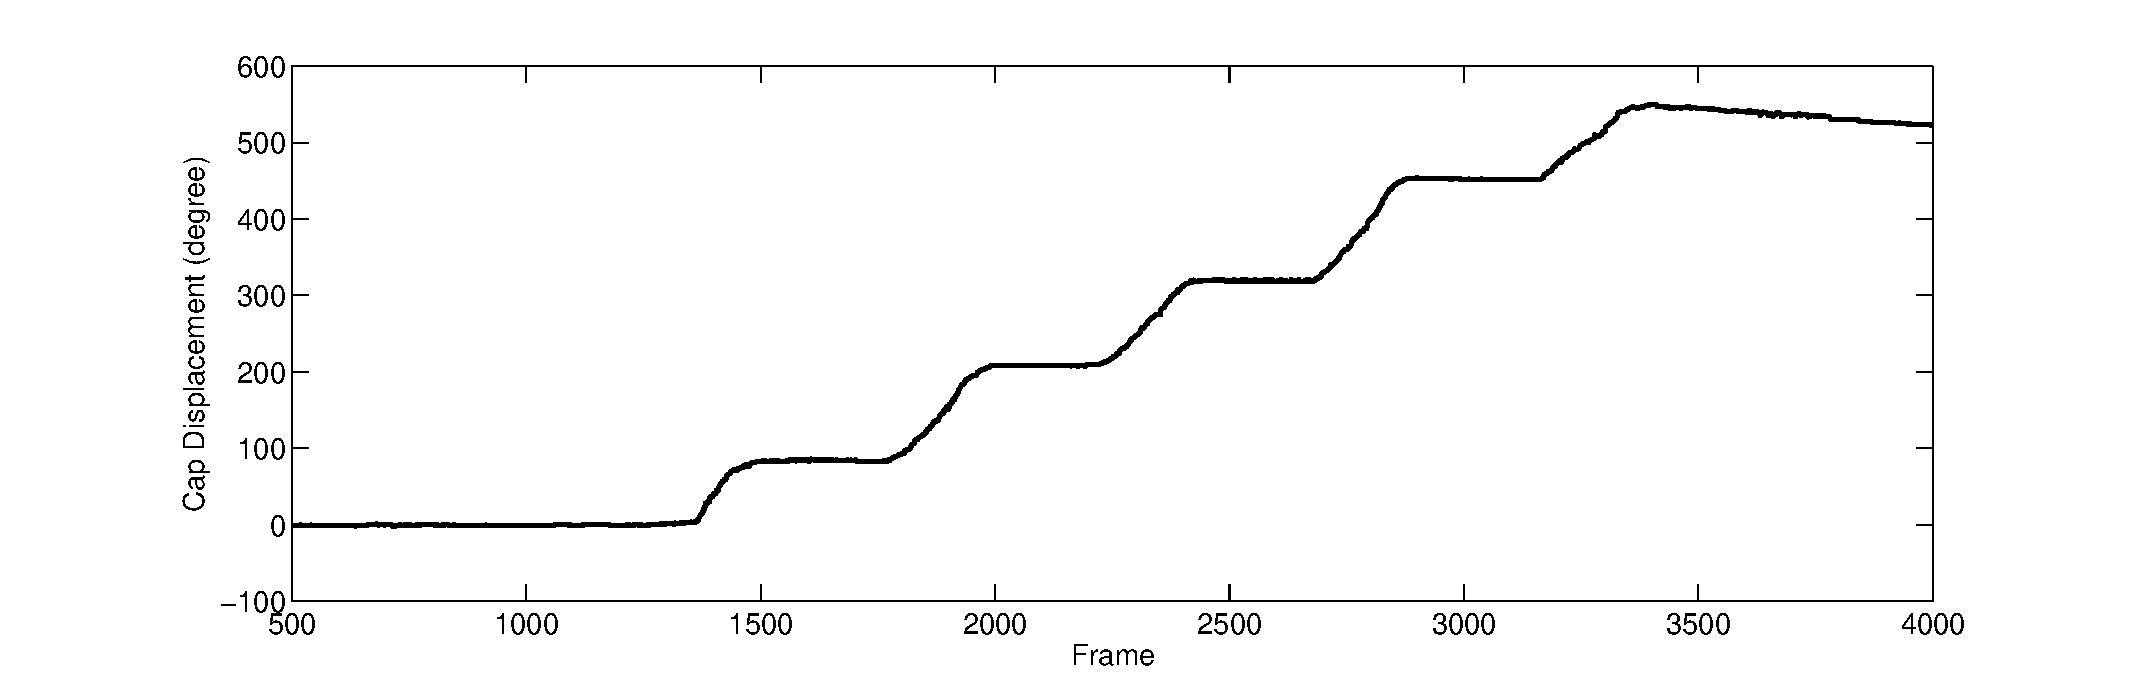
\includegraphics[width=13cm]{./fig/b3c2_5_s.eps}}
  \caption{ \scriptsize{Tracking cap displacement. (a) OptiTrack markers. (b) Cap angular displacement during one demonstration. }
  \label{fig:optitrack}
}
\end{figure}

\subsubsection{Force-Torque Sensor}
\label{ftsensor}
As the movement of the cap is restricted to the rotation along the z-axis, we concern only the torque applied in this direction  (Fig.~\ref{fig:ftsensor}). Other concerned dimension is the force applied in the z direction. The three taps on the cap before each demonstration will create three pulses in the z direction and hence is used for synchronization.

%\begin{itemize}
%  \item Torque in z axis is used as training data \ldots
%  \item Data segmented by torque in z axis \ldots
%\end{itemize}


\begin{figure}
  \centering
  \includegraphics[width=4cm]{./fig/Nano25-E.jpg}
  \vspace{0.2cm}
  \subfloat[\scriptsize{}]  {\includegraphics[width=13cm]{./fig/b3c2_5_T.eps}}
  \caption{ \scriptsize{Force torque sensor. (a) Nano25-E force torque sensor. (b) Exert torque during one demonstration (of b3c2). }
}
\label{fig:ftsensor}
\end{figure}

\subsubsection{Tekscan}
\label{tekscan}
As mentioned in previous section, we use two set of Tekscan to cover the front and the size of the human hand. This enable the demonstrator to use any grasp they like for the task, not restricted to using the first three fingers as most of the other grasp experiment. In each type of grasp, the reading from the patches contacting with the cap are summed and multiplied by their surface area to compute the total grip force (Fig.~\ref{fig:ftsensor}).

\begin{figure}
  \centering
  \includegraphics[width=5cm]{./fig/texscan2.jpg}
  \hspace{0.2cm}
  \subfloat[\scriptsize{}]  {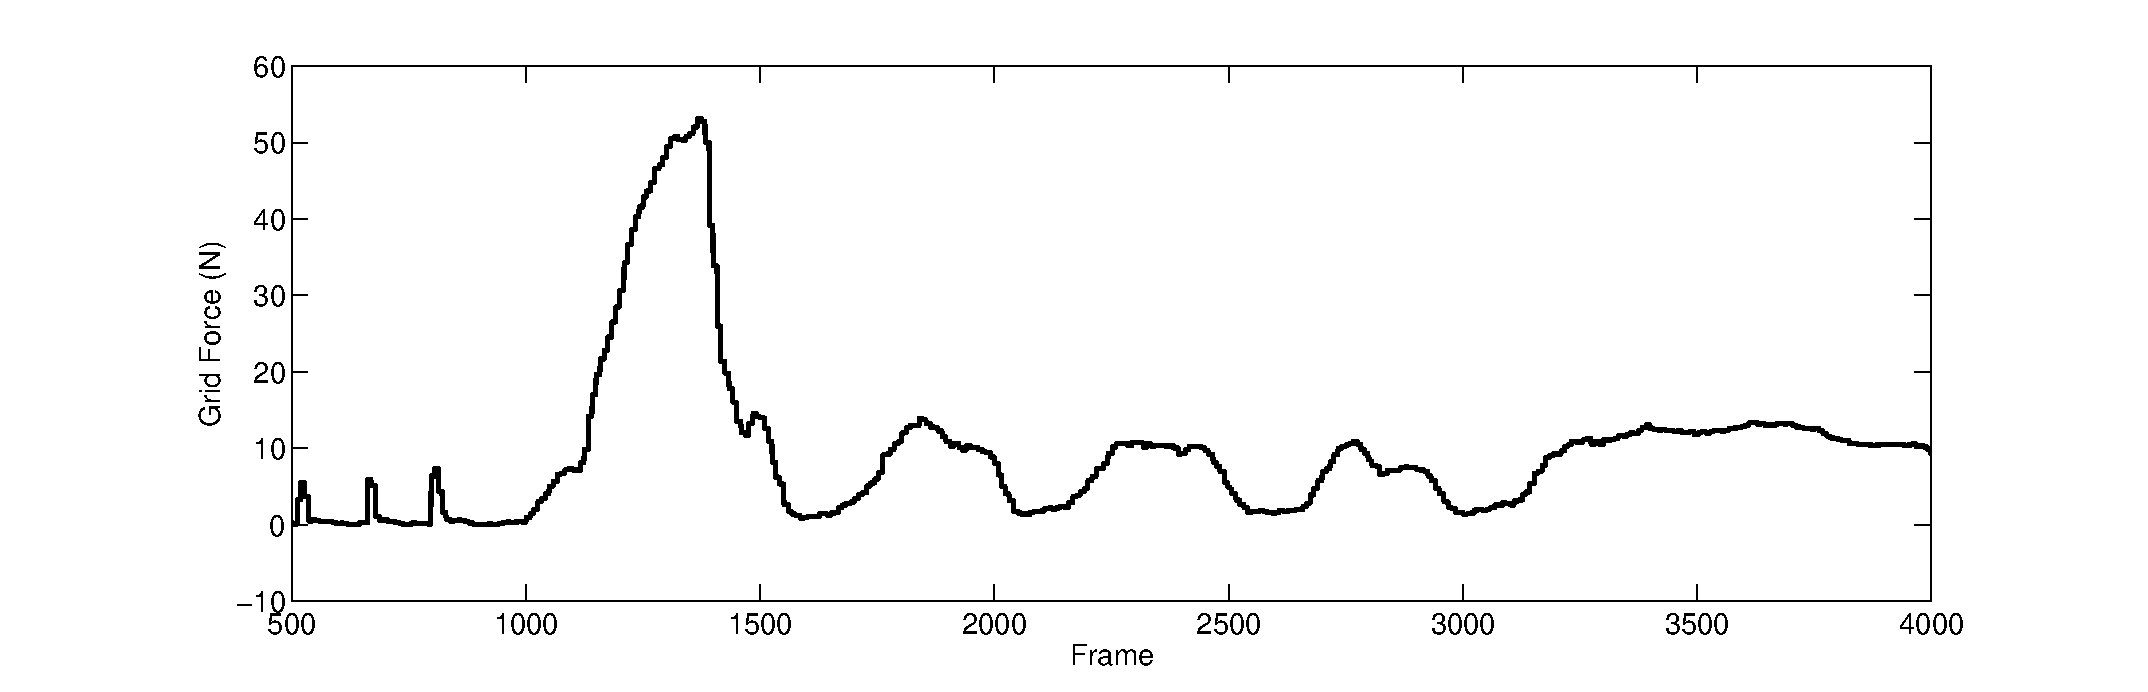
\includegraphics[width=13cm]{./fig/b3c2_5_F.eps}}
  \caption{ \scriptsize{Tracking cap displacement. (a) Tekscan mounted on a glove. (b) Total grib force applied by different parts of the fingers in on demonstration. }
}
\label{fig:ftsensor}
\end{figure}

Data from these three channels is synchronized by aligning the synchronization pulses. The time of the last detected pulse is set to the zero reference point. After synchronization we re-sample all the temporal sequences to 100Hz. Hence each single data point is synchronized. Finally, we filtered the noise by a low pass filter. Fig.~\ref{fig:3channels} shows an example of the data from three different channels.

%\begin{figure}
%  \centering
%  \includegraphics[width=12cm]{./fig/pressure.jpg}
%  \caption{ \scriptsize{Pressure applied by different parts of the fingers.}
%  \label{fig:patch}
%}
%\end{figure}

% filter and resample


\begin{figure*}
  \centering
  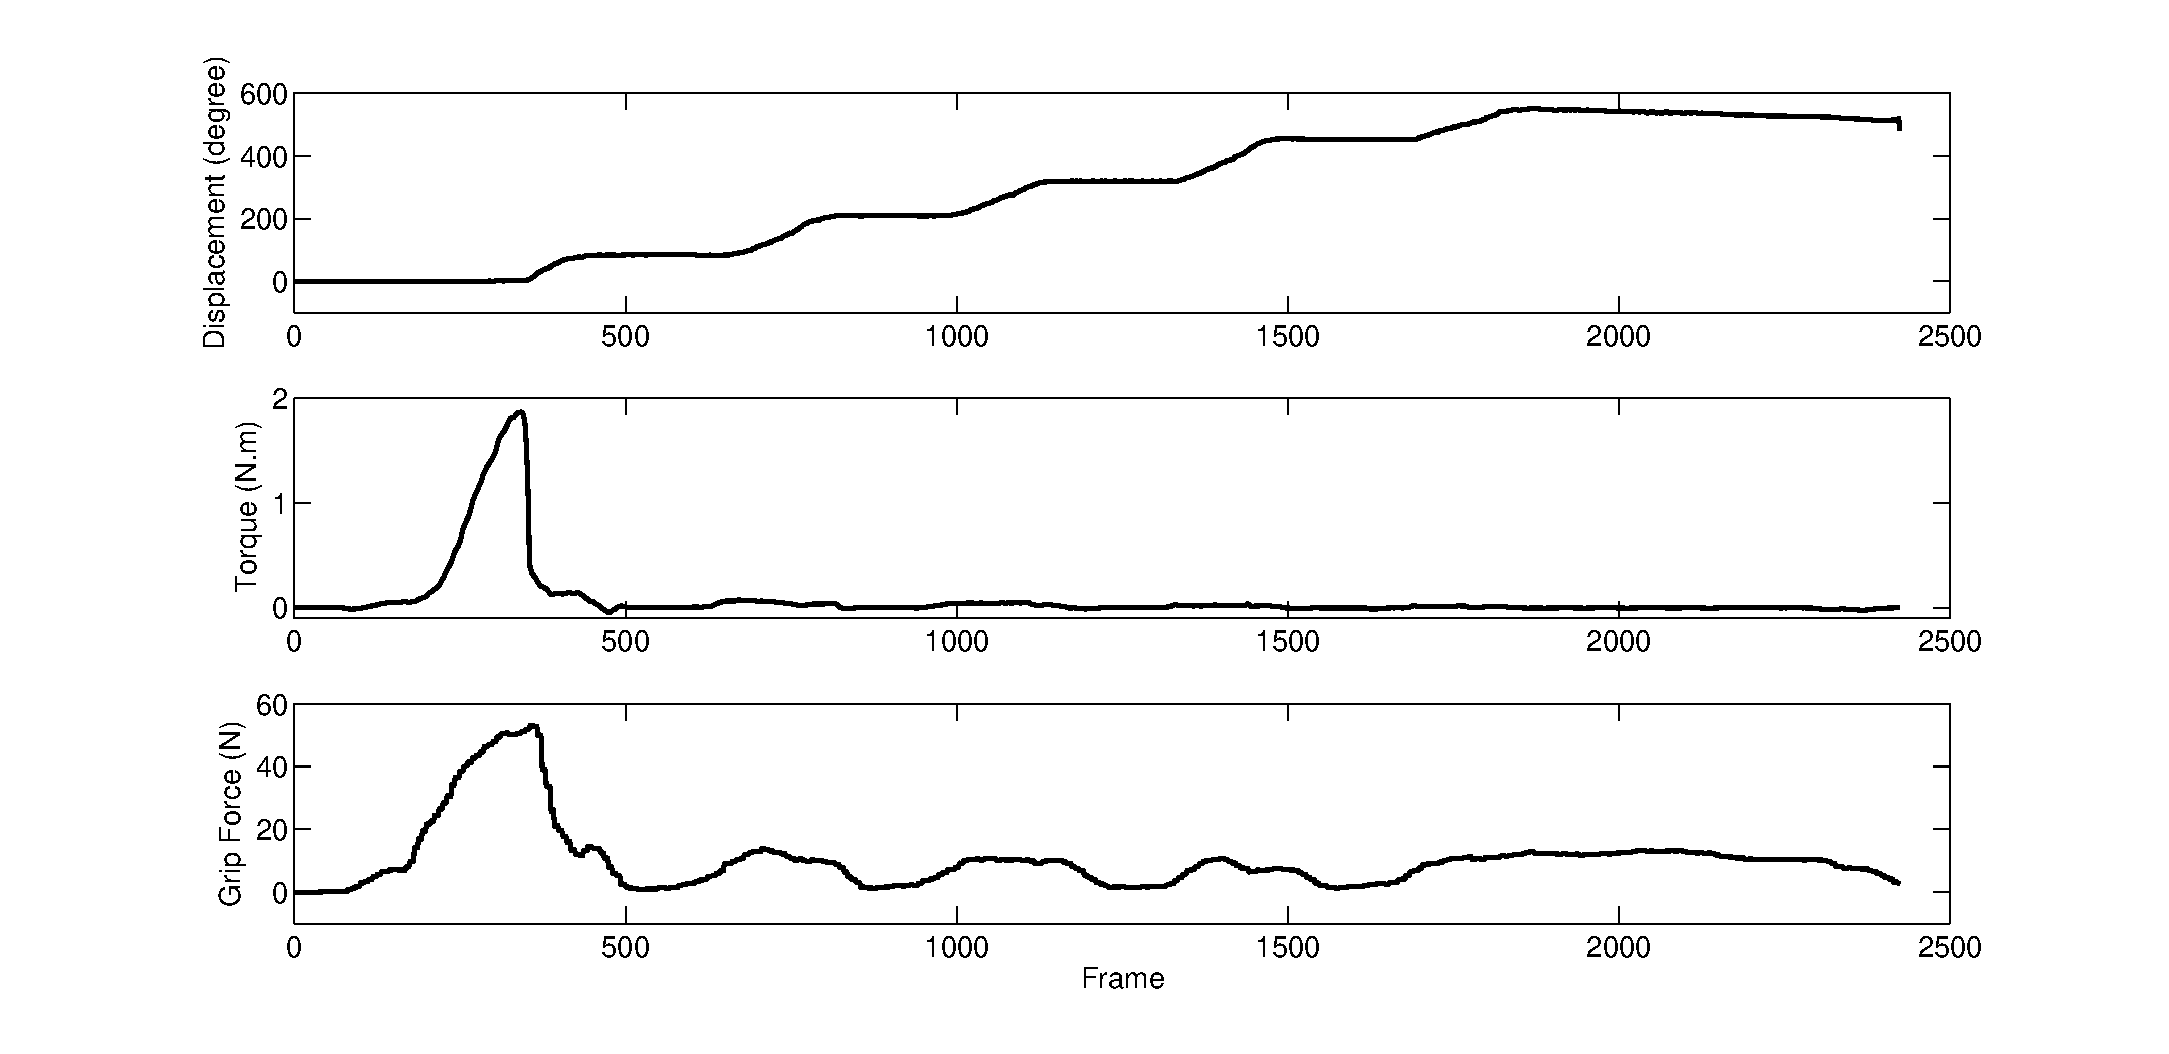
\includegraphics[height=6cm]{./fig/b3c2_5_sTF.eps}
  \caption{ \scriptsize{Aligned data of all three channels.}
}
\label{fig:3channels}
\end{figure*}

% Only turning cycle
In this task we focus on the turning stage of each cycle. More specifically, we focus on the data starts from the moment that the fingers contact the cap and end at the moment that the turning is finished and the cap is released. The reaching and releasing cycles do not involve contact with the environment and hence are not concerned here.
% segmentation is not our job
In order to collect data from only the turning cycles, we trim the data by the contact single: only the sequence with non-zero contact force will be kept.\footnote{In this task the segmentation is done manually. The data can also be segmented by other algorithms but here we do not focus on task segmentation.} The trimmed sequences are labeled by their setups and the order of their appearance, e.g. the 1st cycle of the bottle 1 with cap 3 is labeled by $b1c3_1$.

As can be seem from Fig.~\ref{fig:3channels}, there are dramatic difference between the cycle one and the rest of the cycles: the exert force and torque are much higher in the first cycle than in the other cycles. This is caused by the difference between the static friction and the kinetic friction. At the beginning of the task we have to first break the contact between the bottle and the cap. The friction at this stage is driven by the static friction coefficient. Once the cap starts to move, the friction coefficient between bottle and cap transits to kinetic friction coefficient, which is usually a few times smaller than the static friction coefficient for the same surface. As a result, the torque and hence the grip force required to turn the cap decrease in the later cycles. This phenomenon implies that at lease two modules are needed for this task. In the later section we will discuss these two phases separately and refer the cycle one as ``phase I'' and the later cycles as ``phase II''.

In different demonstrations, the number of cycles used to open the cap is different, varying from four to six. The pattern of the later cycles  are similar as the demonstrator just repeat the same strategy to rotate the cap. For training, we take the first four cycles from each of the demonstration. This results in 84 time series in total for the learning.

%% what was recorded
%In each demonstration, data from first time the hand grab the cap to the cap is finally open and lifted, was record. Opening bottle cap is a cyclic task, each cycle of which includes reaching, turning and releasing stages. Depending on the tightness of the cap, a few cycles need to be done before the bottle is open. In this task we focus on the turning stage of each cycle, which start from the time that the fingers contact the cap and end at the moment that the turning is finished and the cap is released. During the turning cycles, force and torque are applied to the cap in order to break it's contact with the the bottle and the dynamics of the system changes diametrically. Our goal is to learn a model to encode human's strategy to cope with the abruptly changing environment during the turning cycle. The reaching and releasing cycles do not involve contact with the environment and hence we omit them.







\subsection{Learning Modules}
\label{learning}
%\begin{itemize}
%  \item First hierarchical clustering \ldots
%  \item Find out number of models \ldots
%  \item Second build GMM for each of the model \ldots
%\end{itemize}

In this section, we explain how do we encode the training data into a few different modules. As mentioned in Section~\ref{sec:cluster}, the first step is to cluster the data and find out the number of modules required in this task.

\subsubsection{Data clustering}
To cluster the 84 time series $Q\{s,\tau,F\}$ obtained from human demonstration, we first computed the distance between each pair of them by the DTW technique. As this task is time independent, ``warping'' of the data in the dimension of time does not effect the control policy encoded in the time series. The distances between each pair of the time series is shown in the heatmap (Fig.~\ref{fig:heatmap}).

\begin{figure}
\label{heatmap}
  \centering
  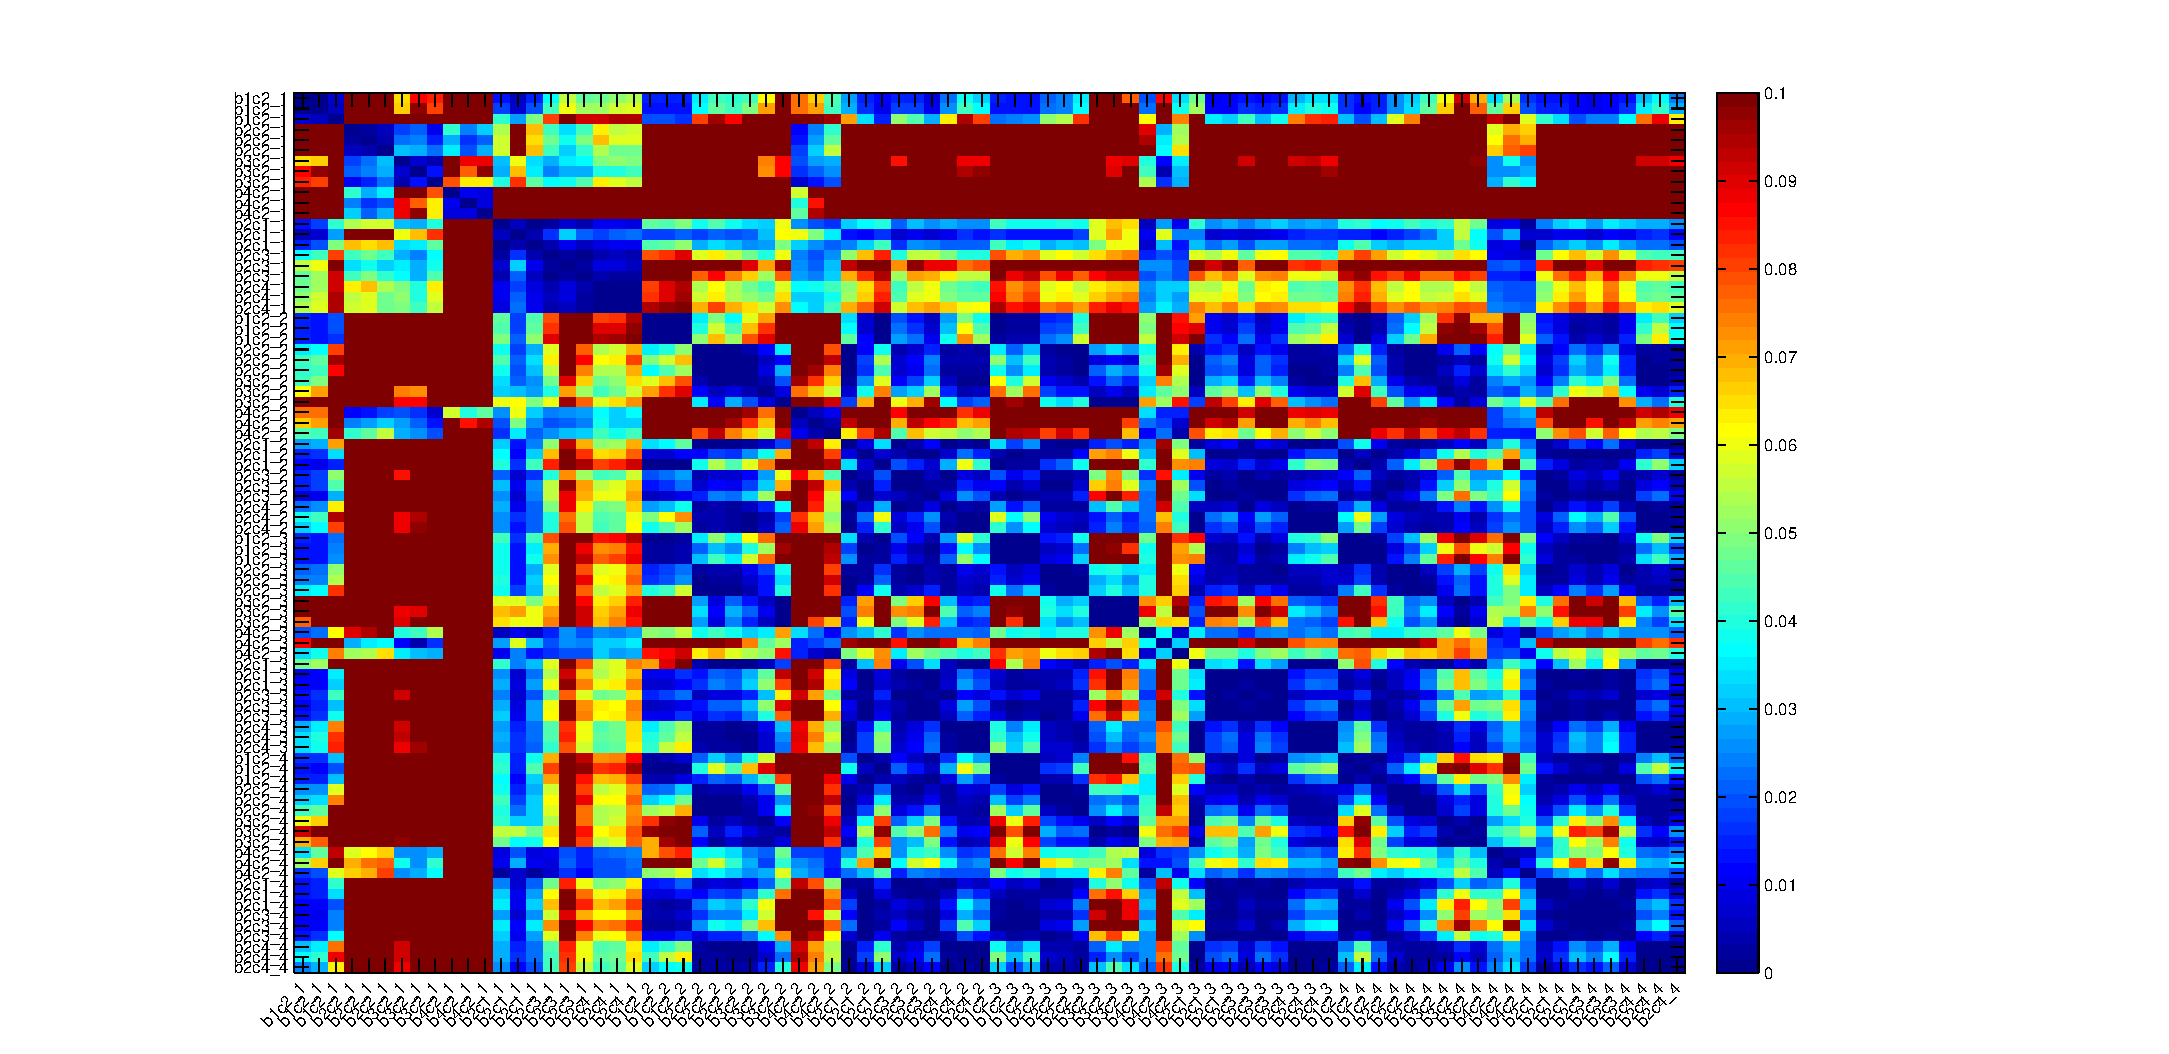
\includegraphics[width=17cm]{./fig/heatmap_all4.eps}
  \caption{ \scriptsize{A heatmap representation of the distances between each pair of time series.}
}
\label{fig:heatmap}
\end{figure}

As mentioned before, the demonstration of each setup is repeated three times and the data from the same setup and same cycle are presumed to belong to the same cluster. To set a threshold for clustering, we check the distances between the time series come from the same setup and the same phase. The largest distance found is 0.04 (normalized) from the $b3c2$ phase 4. We add a $10\%$ margin on this (resulting to 0.044) and use it as the threshold of clustering. The time series distance less than the threshold are grouped into the same cluster. We use the hierarchical agglomerative clustering (Section~\ref{sec:cluster}) to merge the data into different clusters. After 5 times of merging, the clusters are not mergeable and 3 clusters remains.

These three clusters contain the data from:

\begin{enumerate}
\item phase I of $b4c2$ (most difficult bottle), 3 time series;
\item phase I of $b2c2, b3c2, b2c1, b2c3, b2c4$ and phase II of $b4c2$, 24 time series;
\item phase I of $b1c2$ (easiest bottle) and phase II of the other setups, 57 time series.
\end{enumerate}

The result of clustering is shown in Table~\ref{tab:cluster}. This result suggests that human use three different strategies for opening bottles: one for handling the phase I of the most difficult bottle with adhesive materials on the bottle and cap surfaces; one for handling the phase I of most bottles and the phase II of the most difficult bottle; and one for handling the phase I of the lubricated bottle and the phase II of the other bottles. The size of the cap turn out to be playing a less important role in the control strategies. According to this result, we encode these three clusters separately.


\begin{table}
\centering
\renewcommand{\arraystretch}{1.5}
    \begin{tabular}
    %{|>{\centering\arraybackslash}p{2cm}|>{\centering\arraybackslash}p{1.2cm}|>{\centering\arraybackslash}p{1.7cm}|>{\centering\arraybackslash}p{1.2cm}|>{\centering\arraybackslash}p{1.5cm}|>{\centering\arraybackslash}p{1.5cm}|>{\centering\arraybackslash}p{1.7cm}|>{\centering\arraybackslash}p{1.7cm}|>{\centering\arraybackslash}p{0.9cm}|}
    { | c |>{\centering\arraybackslash}p{10cm}|}
    \hline
    Cluster & Member time series \\ \hline
    1       & $b4c2_1$  \\ \hline
    2       & $b2c2_1,b3c2_1,b4c2_2,b4c2_3,b4c2_4,b2c3_1,b2c4_1$  \\ \hline
    3       & $b1c2_1,b1c2_2,b1c2_3,b1c2_4,$
             $  b2c2_2,b2c2_3,b2c2_4, $ \\
    &         $  b3c2_2,b3c2_3,b3c2_4, $
            $  b2c1_2,b2c1_3,b2c1_4, $ \\
    &         $  b2c3_2,b2c3_3,b2c3_4, $
             $  b2c4_2,b2c4_3,b2c4_4$  \\ \hline
    \end{tabular}
\caption{Clustering result}
\label{tab:cluster}
\end{table}

%\begin{figure}
%\label{forcecluster}
%  \centering
%  \includegraphics[width=11cm]{./fig/forcecluster.jpg}
%  \caption{ \scriptsize{Hierarchal clustering result.}
%}
%\end{figure}

\subsubsection{Learning Modules}
\label{sec:module}
We encode the data in each of the module by GMM. As explained in Section~\ref{sec:model}, a forward model and an inverse model are built for each module. The forward model is encoded by the joint distribution $p\{s(t),s(t-1),a(t-1)\mid\Omega_F\}$, while the inverse model is encoded by $p\{s(t),s(t+1),a(t),a(t-1)\mid\Omega_I\}$. For each model, the number of Gaussians is determined by the BIC. We use 25 Gaussian for cluster 1, 40 for cluster 2 and 15 for cluster 3. Their BIC tests are shown in Fig~\ref{fig:bic}.

\begin{figure}
  \centering
  \includegraphics[width=4cm]{./fig/bic_cluster1.eps}
  \includegraphics[width=4cm]{./fig/bic_cluster2.eps}
  \includegraphics[width=4cm]{./fig/bic_cluster3.eps}
  \caption{ \scriptsize{BIC test result for clusters. (a) Cluster 1, (b) Cluster 2, (c) Cluster 3.}
}

\label{fig:bic}
\end{figure}

%\begin{table}
%\centering
%\renewcommand{\arraystretch}{1.5}
%    \begin{tabular}
%    %{|>{\centering\arraybackslash}p{2cm}|>{\centering\arraybackslash}p{1.2cm}|>{\centering\arraybackslash}p{1.7cm}|>{\centering\arraybackslash}p{1.2cm}|>{\centering\arraybackslash}p{1.5cm}|>{\centering\arraybackslash}p{1.5cm}|>{\centering\arraybackslash}p{1.7cm}|>{\centering\arraybackslash}p{1.7cm}|>{\centering\arraybackslash}p{0.9cm}|}
%    { | c | c | c | c | c |}
%    \hline
%    Cluster & Forward Model &  Inverse Model \\ \hline
%    1       & 98.1\%  & 13.8     \\ \hline
%    2             & 92.1\%  & 21.9    \\ \hline
%    3              & 91.0\%  & 16.0    \\ \hline
%    \end{tabular}
%\caption{Number of Gaussians in each GMM}
%\label{tab:GMM}
%\end{table}


\subsection{Generating motor command for manipulation}
\label{sec:command}
Our approach is independent of robot system and can potentially be applied to any robot. We choose to implement this work with a Barrett hand mounted on a KUKA lightweight robot as they are available in our lab. We implement the multiple module system on this platform to enable the robot opening bottle caps.

In this experiment, we control the wrist joint (last joint of KUKA) for producing torque to turn the bottle cap. A force torque sensor is fixed under the bottle to provide torque feedback. Each finger of the Barrett hand is mounted with a $Syntouch$\footnote{http://www.syntouchllc.com/} tactile sensor, which is calibrated to provide contact force information, for the grip force feedback. The cap displacement is measured by the wrist joint displacement, assuming that there is no slip between the fingers and the cap.

The target bottle is fixed on the top of a table with it's cap tighten. The robot is placed above it on a distance that allows a proper grasp on the cap. The Barrett hand then close the fingers until the bottle cap is touched. This position is recorded as the initial position, where the cap displacement is marked as zero. In the experiment we focus on the turning cycle. The releasing and reaching cycles are programmed by opening the fingers and restoring to the initial position.

We first test the model with the trained bottles and then test with two new bottles. With each bottle, the turning-releasing-restoring cycles are repeated four times. Data stream from the sensors are filtered to $100Hz$. Once the turning cycle starts, the forward models take the torque and displacement at the last time step as input, compute the expected displacement of the current time step. These expected displacements are compared with the actual displacement measured at the sensor to evaluate the reliability, expressed as a normalized responsibility factor, of each module. The inverse models take the current displacement, desired next displacement and the previous force and torque as input to compute the a proper action (force and torque) to take on the cap. Each of the three outputs is multiplied with its responsibility factor, and the final output is the sum of the factorized three outputs.

In implementation on a real robot, we found that without putting any restriction of the responsibility factor, it can change rapidly. This is caused by the environmental noise in the sensory input and this result in instability of the control system. We apply a low pass filter on the responsibility factor to reduce the fluctuation. This filtering implies that the real dynamics does not switch from module to another with high frequency, which makes sensor for our task (Fig.~\ref{fig:rf}).


\begin{figure}
  \centering
  \includegraphics[width=2cm]{./fig/void.jpg}
  \caption{ \scriptsize{Filtered responsibility factor. (TODO)}
}
\label{fig:rf}
\end{figure}

Before apply the final output on the robot, a compensational torque is added to it in order to compensate the slag causing by the distortion of the robot hand during turning. The whole control algorithm is shown in algorithm~\ref{code:control}. A set of snapshots of the implementations are shown in Fig.~\ref{fig:demo_train} and~\ref{fig:demo_new}.
Fig.~\ref{fig:demo_result} shows the sensory data from these demonstrations.

\begin{algorithm}
  \caption{Control Algorithm}
  \begin{algorithmic}[1]
    \For{r = 1:4}
    \State REACHING(): Robot move to initial position\;
        \Function{TURNING()}{} %      \Comment{$\oplus$: bit}
          \State Read previous sensor information $\{s_{t-1},\tau_{t-1},F_{t-1}\}$\;
          \For{k=1:3}
            \State $\hat{s}^{k}$ = FORWARD($s_{t-1},T_{t-1},\Omega_I^k$) \;
          \EndFor
          \For{k=1:3}
            \State $\lambda{k}$ = ResponsibilityFactor($\hat{s}^{k},s_t$) \;
          \EndFor
          \State Read current sensor information $\{s_{t}\}$\;
          \For{k=1:3}
            \State $\{a^k\}$ = INVERSE($s*_{t+1},s_t,a_{t-1}$) \;
          \EndFor
          \State $\{a_t\} = \sum_{k=1,2,3}\lambda{k}\{a^k\}$\;\;
          \State Add compensational torque to $\tau_t$\;
          \State Execute motor command $\{a_t\}$ \;
          \State RELEASING(): Release the cap;
        \EndFunction
    \EndFor

    \While{LIFTCAP() is false}
        \State REACHING();
        \State TURNING();
        \State RELEASING();
    \EndWhile

  \end{algorithmic}
  \label{code:control}
\end{algorithm}




%\begin{itemize}
%  \item Demonstration on the learnt bottles \ldots
%  \item Demonstration on a new bottle \ldots
%  \item Filtering noise  \ldots
%  \item different module's rf
%\end{itemize}

\begin{figure}
  \centering
  \includegraphics[width=15cm]{./fig/demo_train.jpg}
  \caption{ \scriptsize{Robot demonstration on opening a trained bottle cap. (TODO)}
}
\label{fig:demo_train}
\end{figure}

\begin{figure}
  \centering
  \includegraphics[width=15cm]{./fig/demo_new.jpg}
  \caption{ \scriptsize{Robot demonstration on opening a new bottle cap. (TODO)}
}
\label{fig:demo_new}
\end{figure}

\begin{figure}
  \centering
  \includegraphics[width=2cm]{./fig/void.jpg}
  \caption{ \scriptsize{Robot demonstration data. (TODO)}
}
\label{fig:demo_result}
\end{figure}

\section{Conclusion and Discussion}
\label{sec:diss}
In this paper we proposed a modular approach for learning manipulation task from human demonstration. We find out the number of modules needed in a task by hierarchical clustering. From each cluster we use forward and inverse model pairs to model the motor control mechanism. The forward models are to predict the effect of the previous motor command, while the inverse models compute a motor command to bring the current state to a desired state. The statical approach enables us to estimate the reliability of the inferences of each module under the current context. The final motor command is the sum of the weighted command from each module. Our experiments verify that by this modular approach, the robot can automatically recognize the current task context and compute motor commands to accomplish a manipulation task, i.e. opening bottle caps.

%We contribute an experimental validation of this approach by learning the human strategy of opening bottle cap. This is a complex manipulation task as the friction between the contact surfaces involve extremely complicated physics. Without detail knowledge of tribology, human success to open many different bottle caps in daily life. We aim to learn this strategy by a modular approach. The human demonstrator demonstrated the task in seven different contexts and we group these demonstrates into three groups. Forward and inverse model pairs are learnt from each group for motor control.

There are many promising directions of further studies of this work. The first is to apply this approach to more contact and friction relative tasks and learn a more general human control strategy to handle the instability caused by friction. To extend our approach to learn tasks involve multiple steps, one could also integrate it with task segmentation technique, to break down the task into atomic steps and recognize the steps needs modular approach. So far we have implement the approach with a task controlled in three dimensions and by three modules. How does the number of modules change according to the dimension of the task is another useful information to reason about.

To summary, tasks involve multiple phases or contexts are hard to implement by a single model. By clustering the control strategies and corresponding task contexts, we are able to focus on each task subspace and build local models. Modular architecture is a practical approach for modeling these tasks. As manipulation usually involves multi-phase friction and multi-body interaction, learning manipulation tasks with a modular approach can simplify the modeling problem in a large extend.
%\begin{itemize}
%  \item Can be used in more complex robot
%  \item if slip can be detected ...
%  \item grasp the cap, studied in another experiment
%\end{itemize}

%During the task, the dynamics of the environment changes abruptly. Figure~/ref{phase12} shows an example of the recorded time sequence of the opening bottle cap task. From the 4 turning cycles we see a dramatic difference between the first cycle and the rest of the cycles. This is not surprise as in the first turning cycle we have to apply a large torque to break the contact between the cap and the bottle, i.e. to overcome the static friction. Once the contact is broken, a much smaller torque is required to rotate the cap, i.e. to overcome the kinema.tic friction.


%% The Appendices part is started with the command \appendix;
%% appendix sections are then done as normal sections
%% \appendix

%% \section{}
%% \label{}

%% If you have bibdatabase file and want bibtex to generate the
%% bibitems, please use
%%
%%  \bibliographystyle{elsarticle-num}
%%  \bibliography{<your bibdatabase>}
\bibliographystyle{elsarticle-num}
\bibliography{multimodel}


%% else use the following coding to input the bibitems directly in the
%% TeX file.

%\begin{thebibliography}{00}
%
%%% \bibitem{label}
%%% Text of bibliographic item
%
%\bibitem{}
%
%\end{thebibliography}

\end{document}
\endinput
%%
%% End of file `elsarticle-template-num.tex'.
